\section{MultiCatch}
Aparentemente esta sendo um recurso pouco utilizado tendo em vista a grande quantidade de reais oportunidades mineradas neste estudo conforme exibido na Figura: \ref{fig:Muticatch}. Foram encotrados ao todo 10368 \textit{trys} que possuem blocos \textit{catchs} repetidos essas ocorrências estão distribuídas em 7297 arquivos totalizando 97347 \acs{LOC}, o teste de  similaridade entre os \textit{catchs} foi realizado através de uma chamada a um método exteno que verificava a igualdade podendo ser facilmente alterado para verificar a similaridade baseando em algum algoritmo existente.

\begin{figure}[h]
	\center
	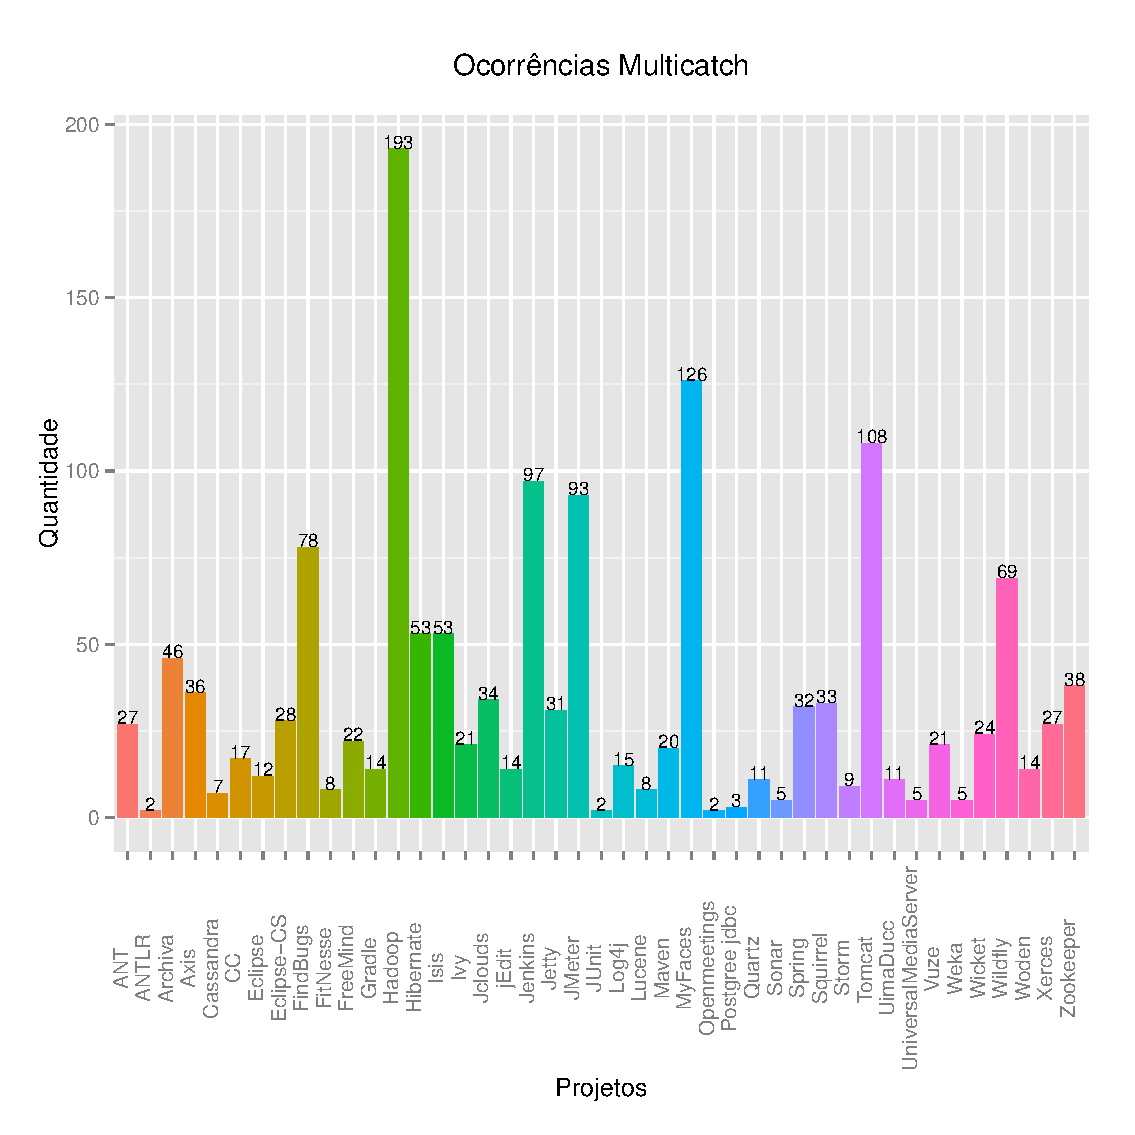
\includegraphics[width=13cm,height=7.8cm]{Imagens/ocorrenciasMulticatch}
	\label{fig:Muticatch}
	\caption{Oportunidades de \textit{Multicatch} nos projetos.}
\end{figure}
		

\begin{lstlisting}
	//              Sem uso de Multicacth 17 LOC
	try {...}
	catch (ConverterNotFoundException ex) {
		PropertyChangeEvent pce =
			new PropertyChangeEvent(this.rootObject, this.nestedPath + propertyName, oldValue, newValue);
		throw new ConversionNotSupportedException(pce, td.getType(), ex);
	}catch (ConversionException ex) {
		PropertyChangeEvent pce =
			new PropertyChangeEvent(this.rootObject, this.nestedPath + propertyName, oldValue, newValue);
		throw new TypeMismatchException(pce, requiredType, ex);
	}catch (IllegalStateException ex) {
		PropertyChangeEvent pce =
			new PropertyChangeEvent(this.rootObject, this.nestedPath + propertyName, oldValue, newValue);
		throw new ConversionNotSupportedException(pce, requiredType, ex);
	}catch (IllegalArgumentException ex) {
		PropertyChangeEvent pce =
			new PropertyChangeEvent(this.rootObject, this.nestedPath + propertyName, oldValue, newValue);
		throw new TypeMismatchException(pce, requiredType, ex);
	}
\end{lstlisting}


\begin{lstlisting}
	//              Com uso de Multicatch 10 LOC
	try {...}
	catch (ConverterNotFoundException ex | IllegalStateException ex) {
		PropertyChangeEvent pce =
			new PropertyChangeEvent(this.rootObject, this.nestedPath + propertyName, oldValue, newValue);
		throw new ConversionNotSupportedException(pce, td.getType(), ex);
	}catch (ConversionException ex | IllegalArgumentException ex) {
		PropertyChangeEvent pce =
			new PropertyChangeEvent(this.rootObject, this.nestedPath + propertyName, oldValue, newValue);
		throw new TypeMismatchException(pce, requiredType, ex);
	}	
\end{lstlisting}

Um simples \textit{refactoring} unindo estes blocos semelhantes por igualdade acarretaria em redução de 68063 \acs{LOC} o que reduz o código duplicado em 70\%, 29284 \acs{LOC}, tornando essa \textit{feature} muito relevante na rescrita de um software. Como exemplo foi utilizado uma classe a \textit{org.springframework.beans.AbstractNestablePropertyAccessor.java} do \textit{Spring 4.2.0.RC2}, onde é possível implantar essa característica de maneira rápida e sem impacto na aplicação, reduzindo em 40\%  o trecho de código.

%Uma análise mais detalhada sobre \textit{JBoss, Spring, Hibernate e Findbugs} totalizando juntos 7778 ocorrências, iniciando na 3.0.0.M1 lançada em junho de 2009 até a mais recente até o momento 4.2.0.RC2. Para uma análise mais criteriosa será elaborada um detalhamento a partir da versão 4.0.0.M1 até a 4.2.0.RC2 totalizando 927 oportunidades de \textit{multicatch} 35\% das ocorrências no \textit{Spring}.\\

A figura: \ref{fig:ocorrenciasMulticatchVersoes} exibe as ocorrências nos projetos mais numerosos do estudo. Onde todas as ocorrências totalizam 17100 \acs{LOC} e após um simples \textit{refactoring} conforme o exemplo anterior obtem-se 5955 \acs{LOC} o que acarreta uma redução da ordem de 65\%.\\

\begin{figure}[h]
	\center
	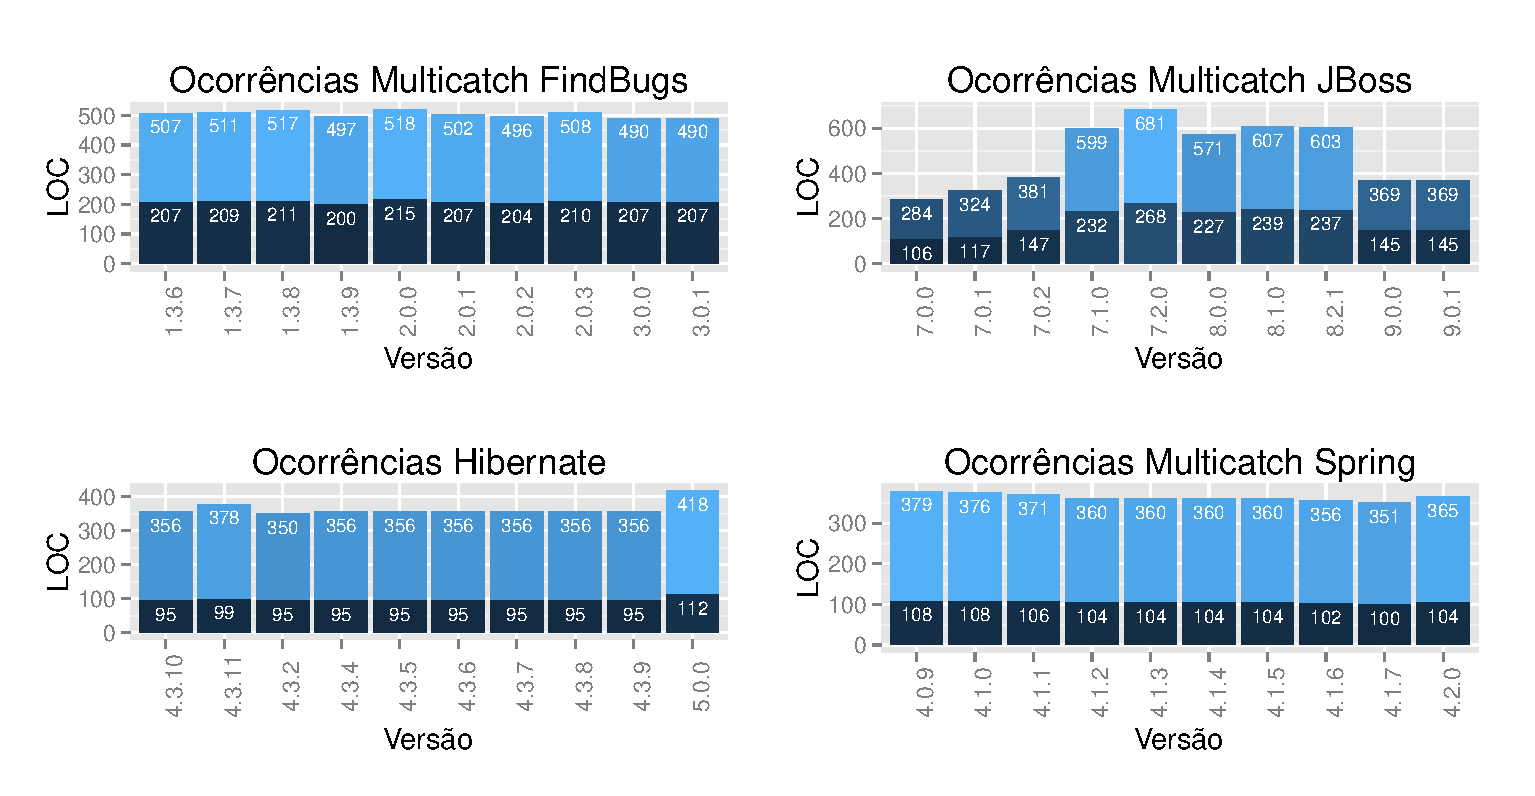
\includegraphics[height=8cm, keepaspectratio]{Imagens/ocorrenciasMulticatchVersoes}
	\label{fig:ocorrenciasMulticatchVersoes}
	\caption{Oportunidades de \textit{Multicatch} nos projetos.}
\end{figure}

